\chapter{Experimental Design and Feasibility}
\label{ch:experiment}

The preceding chapters developed a theoretical framework for the ion energy flux across a plasma sheath, expressed through the Bohm velocity $u_{\mathrm{B}}$, the sheath-edge ion density $n_{\mathrm{i}}$, and the ion velocity distribution function $f_{\mathrm{i}}(v)$ that sets the energy-resolved flux $\Gamma_{E}$ on a bounding surface. A model gains evidentiary weight only when confronted with a controlled, reproducible experiment. This chapter specifies one: a validation plasma source with a characterised operating envelope, optical access for four complementary diagnostics, a staged commissioning sequence, a DOE matrix isolating each control parameter, and a risk register converting feasibility concerns into an auditable, mitigated plan. Every diagnostic here has already been demonstrated in the cited literature; the aim is to show feasibility with present-day technology, within a bounded budget of time and instrumentation.

\section{Controlled Plasma Source for Validation}

\subsection{Rationale for source selection}

A validation experiment must satisfy several simultaneous requirements: bulk parameters ($T_{\mathrm{e}}$, $n_{\mathrm{e}}$, $T_{\mathrm{i}}$, neutral pressure $p_{0}$) independently adjustable enough to span collisionless and weakly collisional sheath regimes; a planar or well-characterised curved sheath boundary so the one-dimensional theory applies without excessive correction; steady-state or quasi-steady operation over the slowest diagnostic's timescale (Thomson scattering needs high density or shot averaging); and generous, unobstructed optical access, since three of the four diagnostics are optical.

A radio-frequency (RF) capacitively or inductively coupled discharge in argon, in a glass/quartz-walled vessel with a biased or floating planar target electrode, satisfies these constraints better than pulsed-power, arc, or high-density magnetised alternatives. Argon is the baseline gas: its atomic structure gives strong, well-catalogued visible transitions for OES, and the metastable $3d\,^{4}\!F_{7/2}$ level of $\mathrm{Ar\,II}$ provides a well-populated lower state for LIF excitation near \SI{668}{\nano\meter} and \SI{675.3}{\nano\meter} \cite{ref0292,ref0300}. A secondary xenon or helium capability cross-checks mass-dependent effects on the Bohm velocity \cite{ref0322}.

\subsection{Discharge architecture and operating envelope}

The reference source is a capacitively coupled RF discharge at \SI{13.56}{\mega\hertz}, with an optional inductive coil for higher-density points, giving access to both a low-density regime characteristic of processing plasmas and a higher-density regime where presheath collisionality is non-negligible, so collisional corrections to the Bohm criterion can be probed rather than asserted. The intended envelope is given in Table~\ref{tab:source-envelope}.

\begin{table}[htbp]
\centering
\caption{Intended operating envelope of the validation plasma source. Ranges are design targets for the bring-up campaign, not measured values.}
\label{tab:source-envelope}
\begin{tabular}{@{}llll@{}}
\toprule
Parameter & Symbol & Range & Notes \\
\midrule
Neutral gas pressure & $p_{0}$ & \SIrange{0.1}{20}{\milli\torr} & Ar primary, Xe/He secondary \\
Forward RF power & $P_{\mathrm{rf}}$ & \SIrange{10}{300}{\watt} & 13.56 MHz, capacitive/ICP \\
Electron density & $n_{\mathrm{e}}$ & \SIrange{e15}{e18}{\per\cubic\meter} & bulk, mid-plane \\
Electron temperature & $T_{\mathrm{e}}$ & \SIrange{1}{6}{\electronvolt} & OES/Thomson cross-check \\
Ion temperature & $T_{\mathrm{i}}$ & \SIrange{0.03}{0.5}{\electronvolt} & LIF-derived \\
Neutral gas temperature & $T_{\mathrm{g}}$ & \SIrange{300}{500}{\kelvin} & wall-limited \\
Target bias & $V_{\mathrm{b}}$ & \SIrange{-200}{50}{\volt} & DC or RF self-bias \\
Optional axial field & $B$ & \SIrange{0}{100}{\milli\tesla} & solenoid, Chodura studies \\
\bottomrule
\end{tabular}
\end{table}

This envelope is chosen so the ratio of Debye length to neutral collision mean free path spans roughly two orders of magnitude, allowing both the collisionless-sheath limit and collisional presheath broadening to be reached in one apparatus:

\begin{equation}
\lambda_{\mathrm{D}} = \left( \frac{\varepsilon_{0} k_{\mathrm{B}} T_{\mathrm{e}}}{n_{\mathrm{e}} e^{2}} \right)^{1/2},
\label{ch20-eq:debye}
\end{equation}

which ranges from approximately \SI{30}{\micro\meter} at the highest density to several hundred micrometres at the lowest, always small compared with the \SIrange{5}{15}{\centi\meter} vessel dimension, so quasineutrality holds outside a thin boundary layer.

\subsection{Bulk and boundary parameters relevant to the sheath}

The energy flux carried by ions across the sheath edge is set by the ion density and characteristic velocity, together with the shape of the ion velocity distribution. In the cold-ion, collisionless-sheath picture the flux is fixed by the Bohm velocity,

\begin{equation}
u_{\mathrm{B}} = \left( \frac{k_{\mathrm{B}} T_{\mathrm{e}}}{m_{\mathrm{i}}} \right)^{1/2},
\label{ch20-eq:bohm}
\end{equation}

with flux density $\Gamma = n_{\mathrm{i}} u_{\mathrm{B}}$, $n_{\mathrm{i}}$ the ion density at the sheath-presheath boundary (customarily $n_{\mathrm{i}} \approx 0.5\,n_{\mathrm{e},0}$). The energy-resolved flux central to this monograph weights each ion's kinetic energy by the local flux contribution of $f_{\mathrm{i}}(v)$,

\begin{equation}
\Gamma_{E} = \int_{0}^{\infty} \tfrac{1}{2} m_{\mathrm{i}} v^{2}\, v\, f_{\mathrm{i}}(v)\, \mathrm{d}v ,
\label{ch20-eq:gammaE}
\end{equation}

so measuring $\Gamma_{E}$ requires independent measurement of $n_{\mathrm{e}}$ (or $n_{\mathrm{i}}$), $T_{\mathrm{e}}$, and the full shape of $f_{\mathrm{i}}(v)$, not a single moment such as $T_{\mathrm{i}}$. This dictates the four-diagnostic suite: OES and interferometry recover $T_{\mathrm{e}}$ and $n_{\mathrm{e}}$ economically, LIF recovers the shape of $f_{\mathrm{i}}(v)$ to evaluate Equation~\eqref{ch20-eq:gammaE} directly, and Thomson scattering gives a first-principles cross-check free of atomic-physics assumptions.

\section{Optical Access Geometry and Constraints}

\subsection{Port layout}

All four diagnostics are line-of-sight optical techniques, and their joint operation on a single vessel imposes a port-placement constraint resolved at the design stage. The reference vessel is a six-way-cross or octagonal chamber approximately \SI{30}{\centi\meter} in diameter, with fused-silica or sapphire viewports transmitting from the near-ultraviolet (two-photon LIF, \SIrange{200}{230}{\nano\meter}) through the visible (OES, single-photon LIF, Thomson collection) into the near-infrared (\SI{1064}{\nano\meter} Nd:YAG for Thomson), plus dielectric/polymer windows for interferometry. A schematic layout is shown in Figure~\ref{fig:ports}.

\begin{figure}[htbp]
\centering
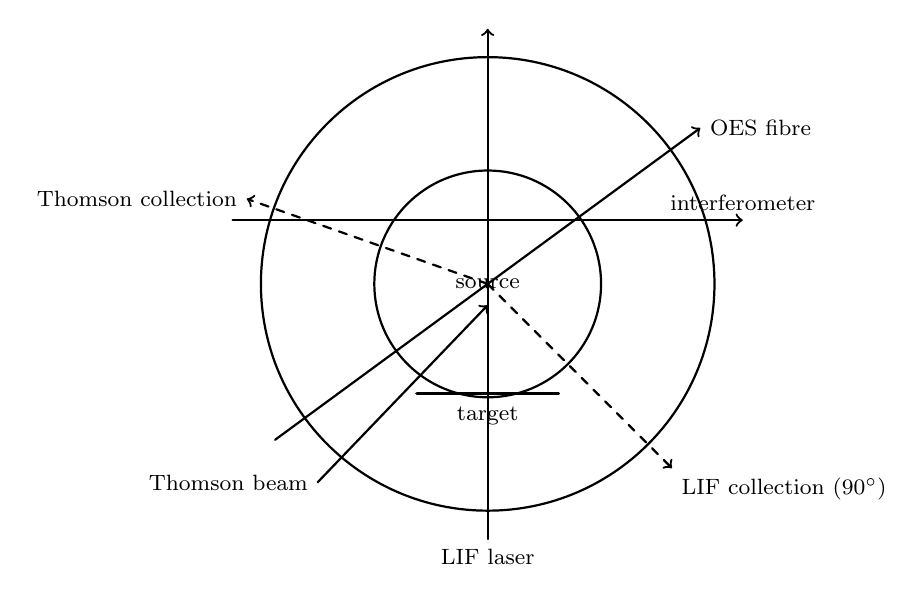
\begin{tikzpicture}[scale=0.9, line cap=round, line join=round]
 \draw[thick] (0,0) circle (3.2);
 \draw[thick, fill=white] (0,0) circle (1.6);
 \node at (0,0) {\footnotesize source};

 \draw[thick,->] (-3.6,0.9) -- (3.6,0.9);
 \node[anchor=south] at (3.6,0.9) {\footnotesize interferometer};

 \draw[thick,->] (-3.0,-2.2) -- (3.0,2.2);
 \node[anchor=west] at (3.0,2.2) {\footnotesize OES fibre};

 \draw[thick,->] (0,-3.6) -- (0,3.6);
 \node[anchor=north] at (0,-3.6) {\footnotesize LIF laser};
 \draw[thick,dashed,->] (0,0) -- (2.6,-2.6);
 \node[anchor=north west] at (2.6,-2.6) {\footnotesize LIF collection ($90^{\circ}$)};

 \draw[thick,->] (-2.4,-2.8) -- (0,-0.3);
 \node[anchor=east] at (-2.4,-2.8) {\footnotesize Thomson beam};
 \draw[thick,dashed,->] (0,0) -- (-3.4,1.2);
 \node[anchor=east] at (-3.4,1.2) {\footnotesize Thomson collection};

 \draw[very thick] (-1.0,-1.55) -- (1.0,-1.55);
 \node[anchor=north] at (0,-1.6) {\footnotesize target};
\end{tikzpicture}
\caption{Schematic (illustrative, not to scale) top-view port layout for simultaneous optical access. Solid arrows denote beam injection or line-of-sight collection; dashed arrows denote scattered/fluorescence collection at a fixed angle relative to the corresponding beam. The inner circle marks the bulk-plasma region; the target electrode subtends the lower sheath boundary.}
\label{fig:ports}
\end{figure}

The layout separates four independent optical axes: a horizontal chord for line-integrated interferometry; a diagonal chord for OES fibre collection avoiding the target and stray light from the biased electrode; a vertical axis for LIF laser injection above the target, with fluorescence collected at \SI{90}{\degree}; and an oblique axis for the Thomson probe beam, also collected at \SI{90}{\degree}. This minimises overlap between the collection solid angle and the reflected or forward-scattered injected beam, orders of magnitude more intense than the signal of interest -- for Thomson scattering the stray-light-to-signal ratio can exceed $10^{6}$--$10^{8}$ in low-density, low-temperature plasmas \cite{ref0357,ref0360}.

\subsection{Constraints from stray light, window fouling, and \'etendue}

Three constraints dominate the optical design. Stray-light rejection: Thomson scattering is photon-starved, and modest stray laser light from walls, windows, or the target electrode can overwhelm the signal; mitigated with baffled Brewster-angle beam dumps, anti-reflection-coated windows, and a triple-grating or notch-filtered spectrometer \cite{ref0355,ref0362}. Window fouling: sputtered material deposits on viewports, degrading transmission non-uniformly; Thomson scattering sits behind a retractable shutter closed except during acquisition, recalibrated via a reference Rayleigh gas fill \cite{ref0355,ref0384}. \'Etendue matching: collection optics must match the scattering volume and detector acceptance, trading spatial resolution against signal, using $f/4$--$f/6$ optics imaging a volume of order \SI{1}{\milli\meter}, small against the presheath but large enough for adequate signal.

\subsection{Spatial resolution and alignment tolerances}

Because ion energy flux is a boundary-layer quantity, the diagnostics must resolve $n_{\mathrm{e}}(x)$, $T_{\mathrm{e}}(x)$, and $f_{\mathrm{i}}(v;x)$ versus distance $x$ from the target, fine compared with the presheath scale length. The LIF collection optics sit on a motorised stage with \SI{50}{\micro\meter} repeatability, scanning to within approximately \SI{1}{\milli\meter} of the target, the limit set by stray reflected laser light. Interferometry, being line-integrated, does not resolve the sheath directly; its role is a robust line-averaged bulk density against which the spatially resolved density from OES and Thomson scattering is cross-checked. Alignment uses a retroreflected HeNe laser before each session, with registration verified to better than \SI{0.2}{\milli\meter}.

\section{Staged Bring-Up: OES and Interferometry First, then LIF, then Thomson Scattering}
\label{sec:staged-bringup}

A central design decision is to commission the four diagnostics in a deliberate sequence, ordered by increasing technical risk. OES and interferometry are passive or low-power, requiring no pulsed-laser infrastructure, and provide an immediate estimate of $n_{\mathrm{e}}$ and $T_{\mathrm{e}}$ against which LIF and Thomson are later validated.

\subsection{Stage 1: Optical emission spectroscopy and interferometry}

OES is commissioned first because it requires no active probe beam, is immune to the alignment and stray-light difficulties of later stages, and has an extensive track record in noble-gas discharges spanning this envelope \cite{ref0231,ref0237}. The method rests on a collisional-radiative (CR) treatment of excited-state population balance: for two lines populated predominantly by electron-impact excitation from the ground or a metastable state, the intensity ratio is a function of $T_{\mathrm{e}}$ alone,

\begin{equation}
\frac{I_{p}}{I_{q}} = \frac{A_{p} \, n_{\mathrm{e}} \, X_{p}(T_{\mathrm{e}})}{A_{q} \, n_{\mathrm{e}} \, X_{q}(T_{\mathrm{e}})} = \frac{A_{p}\,X_{p}(T_{\mathrm{e}})}{A_{q}\,X_{q}(T_{\mathrm{e}})},
\label{eq:oes-ratio}
\end{equation}

where $A_{p}$ is the Einstein $A$ coefficient and $X_{p}(T_{\mathrm{e}})$ the electron-impact excitation rate coefficient into level $p$, from convolving the cross section with an assumed (typically Maxwellian) electron energy distribution. Since $n_{\mathrm{e}}$ cancels when both lines share the dominant excitation pathway, Equation~\eqref{eq:oes-ratio} yields $T_{\mathrm{e}}$ from intensity ratios alone, validated from RF and microwave sources to Hall-effect thrusters \cite{ref0245,ref0256}. Absolute $n_{\mathrm{e}}$ is recovered from a single line intensity via the full CR balance, at lower confidence.

Line-integrated microwave or infrared interferometry runs in parallel with OES, providing an independent, model-free line-averaged $n_{\mathrm{e}}$ anchoring the OES density scale. For a probe of wavelength $\lambda$ traversing path length $L$ through density $n_{\mathrm{e}}(x)$ well below critical density $n_{\mathrm{c}} = \varepsilon_{0} m_{\mathrm{e}} \omega^{2}/e^{2}$, the refractive index is $n_{\mathrm{r}}(x) \approx 1 - n_{\mathrm{e}}(x)/(2 n_{\mathrm{c}})$, giving phase shift

\begin{equation}
\Delta \phi = \frac{2\pi}{\lambda} \int_{0}^{L} \bigl[1 - n_{\mathrm{r}}(x)\bigr] \, \mathrm{d}x = r_{\mathrm{e}} \lambda \int_{0}^{L} n_{\mathrm{e}}(x) \, \mathrm{d}x,
\label{ch20-eq:interferometry}
\end{equation}

where $r_{\mathrm{e}} = e^{2}/(4\pi\varepsilon_{0} m_{\mathrm{e}} c^{2}) \approx \SI{2.818e-15}{\meter}$ is the classical electron radius. The phase shift is directly proportional to the line-integrated density, independent of any assumed electron energy distribution -- why interferometry is a valuable cross-check on the OES scale, demonstrated at comparable density and geometry \cite{ref0400}, with heterodyne variants giving phase resolution and vibration immunity, and dispersion variants suppressing mechanical path-length drift \cite{ref0417}.

Stage 1 is complete when OES- and interferometry-derived values are reproducible (day-to-day repeatability better than \SI{15}{\percent}) and agree within the expected geometric factor.

\subsection{Stage 2: Laser-induced fluorescence}

LIF is introduced only after Stage 1 establishes a cross-checked density and temperature scale against which the LIF-derived distribution can be sanity-checked. LIF is central to this programme: it alone measures the full shape of $f_{\mathrm{i}}(v)$, enabling direct evaluation of Equation~\eqref{ch20-eq:gammaE} rather than a Maxwellian-equivalent moment.

The technique exploits the Doppler shift of a narrow-linewidth, tunable laser resonant with an ion transition: an ion of velocity $v$ is excited only when

\begin{equation}
\nu = \nu_{0} \left( 1 + \frac{v}{c} \right),
\label{eq:doppler}
\end{equation}

with $\nu_{0}$ the rest-frame transition frequency. Scanning the laser across the Doppler-broadened profile and recording fluorescence $S(\nu)$ maps the one-dimensional ion velocity distribution along the probe direction, up to instrumental broadening removed by deconvolution,

\begin{equation}
f_{\mathrm{i}}(v) \; \propto \; \bigl[ S(\nu) \ast g_{\mathrm{laser}}^{-1} \bigr] \Big|_{\nu = \nu_{0}(1+v/c)},
\label{eq:lif-inversion}
\end{equation}

where $g_{\mathrm{laser}}$ is the laser lineshape and $\ast^{-1}$ denotes deconvolution, described in the foundational and review literature \cite{ref0292,ref0300}.

For argon, the reference scheme excites the metastable $3d\,^{4}\!F_{7/2}$ state of $\mathrm{Ar\,II}$ at \SI{668.6}{\nano\meter}, collecting fluorescence on the cascade transition near \SI{442.6}{\nano\meter}, validated in RF and Hall-thruster plasmas with sheath-adjacent geometry \cite{ref0322}.

Three technical risks specific to LIF are addressed at the design stage: excitation saturation, distorting the lineshape and biasing the inferred temperature, checked via a saturation curve (fluorescence versus laser power) at each point \cite{ref0292}; spatial inhomogeneity of laser intensity and finite \'etendue overlap between beam and collection optics, corrected using established normalisation procedures \cite{ref0304}; and, in a magnetised configuration ($B \neq 0$), laser/velocity-space misalignment, modelled to set an alignment tolerance for solenoid runs.

Stage 2 is complete when the LIF-derived ion density (integrated $f_{\mathrm{i}}(v)$, calibrated against Stage 1 $n_{\mathrm{e}}$ under quasineutrality) agrees with the Stage 1 scale, and the extracted ion temperature and drift vary smoothly with $x$ across the presheath-to-sheath transition.

\subsection{Stage 3: Thomson scattering}

Thomson scattering is introduced last, being the most demanding diagnostic: it requires a high-energy pulsed laser, a stray-light-suppressed collection path, and single-photon-counting detection near the lower end of Table~\ref{tab:source-envelope}. Its role is essential: it is the only diagnostic whose interpretation does not rely on an assumed CR model or electron energy distribution, and is the ultimate arbiter of the scale against which OES and LIF are validated \cite{ref0383,ref0384}.

For non-relativistic electrons and incident wavelength $\lambda_{0}$, in the incoherent-scattering regime the scattered spectral power at angle $\theta$ has an approximately Gaussian profile, Doppler-broadened by thermal electron motion, whose FWHM gives $T_{\mathrm{e}}$ via

\begin{equation}
\Delta \lambda_{1/2} = 2 \lambda_{0} \sin\!\left(\frac{\theta}{2}\right) \left( \frac{8 \ln 2 \, k_{\mathrm{B}} T_{\mathrm{e}}}{m_{\mathrm{e}} c^{2}} \right)^{1/2},
\label{eq:thomson-width}
\end{equation}

so $T_{\mathrm{e}}$ is obtained directly from spectral width, unlike the OES method of Equation~\eqref{eq:oes-ratio}. The scattered power collected within $\mathrm{d}\Omega$ from a probe volume of length $L$ and incident power $P_{\mathrm{L}}$ is

\begin{equation}
P_{\mathrm{s}} = P_{\mathrm{L}} \, n_{\mathrm{e}} \, \sigma_{\mathrm{T}} \, L \, \frac{\mathrm{d}\Omega}{4\pi} \, \eta_{\mathrm{opt}},
\label{eq:thomson-power}
\end{equation}

with $\sigma_{\mathrm{T}} \approx \SI{6.65e-29}{\meter\squared}$ the Thomson cross section and $\eta_{\mathrm{opt}}$ the net transmission-and-detection efficiency; $n_{\mathrm{e}}$ is recovered once $\eta_{\mathrm{opt}}$ is established via a Raman or Rayleigh calibration shot, from early demonstrations through modern portable, high-repetition-rate systems \cite{ref0355,ref0357,ref0383,ref0384}.

At the lower density end, $n_{\mathrm{e}} \sim \SI{e15}{\per\cubic\meter}$, Equation~\eqref{eq:thomson-power} predicts small photon counts per pulse, and the dominant challenge is distinguishing genuine signal from Rayleigh scattering and stray light -- addressed by triple-grating/notch-filter rejection and attention to ponderomotive perturbations at the intensities needed \cite{ref0360,ref0362}. The design accumulates signal over many shots in a steady-state or periodically pulsed mode \cite{ref0357}.

Stage 3 is complete when Thomson-derived $(n_{\mathrm{e}}, T_{\mathrm{e}})$ agrees with the Stage 1 and 2 values at a representative subset of the envelope, closing the cross-validation loop and fixing the parameters that enter Equation~\eqref{ch20-eq:gammaE} alongside the LIF-derived ion velocity distribution.

\section{Design of Experiments}

\subsection{Independent and dependent variables}

The campaign is structured as a factorial DOE rather than an unstructured sweep, so the influence of each independent variable is isolated and interaction effects (e.g.\ pressure and RF power, both affecting $T_{\mathrm{e}}$) are resolved rather than confounded. The independent variables are gas species and pressure $p_{0}$, RF power $P_{\mathrm{rf}}$, target bias $V_{\mathrm{b}}$, and, in the magnetised sub-campaign, axial field $B$. The dependent variables are OES- and Thomson-derived $T_{\mathrm{e}}$, $n_{\mathrm{e}}$, the interferometric line-averaged density, and the LIF-derived $f_{\mathrm{i}}(v;x)$, from which $u_{\mathrm{B}}$, $\lambda_{\mathrm{D}}$, and $\Gamma_{E}$ follow.

\subsection{Measurement matrix}

Table~\ref{tab:doe-matrix} summarises the core measurement matrix. Each row is an operating point visited with the full Stage-1/2/3 suite; the matrix is a partial factorial (central composite-like) rather than a full factorial, keeping campaign duration tractable while retaining the ability to fit a response surface for $\Gamma_{E}(p_{0}, P_{\mathrm{rf}}, V_{\mathrm{b}}, B)$.

\begin{table}[htbp]
\centering
\caption{Representative measurement matrix. ``Baseline'' denotes the mid-envelope reference point; other rows vary one or two factors from baseline to isolate their effects on $\Gamma_{E}$. All rows use the full Stage 1--3 diagnostic suite.}
\label{tab:doe-matrix}
\begin{tabular}{@{}lccccl@{}}
\toprule
Run set & $p_{0}$ & $P_{\mathrm{rf}}$ & $V_{\mathrm{b}}$ & $B$ & Purpose \\
\midrule
Baseline & mid & mid & mid & 0 & reference point, repeatability \\
Pressure scan & low--high & mid & mid & 0 & collisionality dependence \\
Power scan & mid & low--high & mid & 0 & $T_{\mathrm{e}}$, $n_{\mathrm{e}}$ dependence \\
Bias scan & mid & mid & low--high & 0 & sheath-voltage dependence \\
Field scan & mid & mid & mid & 0--max & Chodura/magnetised presheath \\
Gas-species check & Xe, He & mid & mid & 0 & mass dependence of $u_{\mathrm{B}}$ \\
Corner points & low/high & low/high & mid & 0 & interaction terms \\
Repeatability & mid & mid & mid & 0 & day-to-day, operator-to-operator \\
\bottomrule
\end{tabular}
\end{table}

The pressure scan targets the collisionless-to-collisional transition, correlating ion-neutral collision frequency (from $p_{0}$, $T_{\mathrm{g}}$, and known charge-exchange cross sections) against any departure of $f_{\mathrm{i}}(v)$ from the collisionless prediction. The bias scan is central to the energy flux question, since $V_{\mathrm{b}}$ sets the sheath potential drop and terminal ion impact energy, spanning a near-floating, low-flux regime to a strongly biased, high-flux regime resembling sputtering. The gas-species check exploits $u_{\mathrm{B}} \propto m_{\mathrm{i}}^{-1/2}$: switching argon ($m_{\mathrm{i}} \approx \SI{40}{u}$) for helium ($m_{\mathrm{i}} \approx \SI{4}{u}$) at fixed $T_{\mathrm{e}}$ should shift the LIF-derived ion velocity by a factor close to $\sqrt{10}$, a model-independent falsifiability test.

\subsection{Controls and cross-validation}

Since this is a physical measurement campaign, ``controls'' mean internal consistency checks and null tests. Four are built in: the triple cross-check of $(n_{\mathrm{e}}, T_{\mathrm{e}})$ across OES, interferometry, and Thomson scattering (Section~\ref{sec:staged-bringup}), a redundant measurement by methods with independent error budgets so single-diagnostic bias is detectable as disagreement; the quasineutrality closure test, comparing LIF-derived ion density against Stage 1/3 electron density, checking LIF absolute calibration (otherwise a relative, lineshape-only measurement); a laser-off, plasma-on null run at every LIF/Thomson point, characterising plasma self-emission subtracted from the laser-on signal \cite{ref0304,ref0355}; and a laser-on, plasma-off null run characterising stray-light and window-fluorescence background. Repeatability runs (Table~\ref{tab:doe-matrix}) are distributed throughout the campaign, not concentrated at start or end, so slow drift in conditioning, transmission, or alignment is captured over time rather than aliased into the results.

\section{Risk Register and Mitigation; Feasibility Argument}

\subsection{Risk register}

Table~\ref{tab:risk-register} enumerates the principal technical risks, with assessed likelihood, impact on the validity of the final measurement, and the mitigation adopted at the design stage; each entry maps onto a design decision already embedded in the apparatus or procedure.

\begin{table}[htbp]
\centering
\small
\begin{tabularx}{\textwidth}{@{}lccX@{}}
\toprule
Risk & Likelihood & Impact & Mitigation \\
\midrule
Thomson signal buried in stray light at low $n_{\mathrm{e}}$ & high & high & triple-grating/notch rejection, beam dumps, shot accumulation, Rayleigh calibration \cite{ref0360,ref0362} \\
LIF saturation distorts $f_{\mathrm{i}}(v)$ & medium & high & saturation curve at each point; operate on linear branch \cite{ref0292} \\
Window fouling degrades absolute calibration & high & medium & retractable shutters; periodic Rayleigh recalibration \\
OES CR-model systematic bias in $n_{\mathrm{e}}$ & medium & medium & anchor to interferometric line-average \cite{ref0231,ref0237} \\
Diagnostic disagreement (OES vs.\ Thomson vs.\ LIF closure) & medium & high & staged bring-up exposes disagreement early \\
Mechanical/thermal drift of interferometer path & medium & low & dispersion interferometer configuration \cite{ref0417} \\
Laser-induced perturbation of plasma (ponderomotive) at Thomson intensities & low & medium & operate below documented perturbation threshold \cite{ref0360} \\
Alignment drift across four optical axes over campaign & medium & medium & HeNe retroreflection check each session \\
Magnetised-mode disalignment bias in LIF & low & medium & quantitative disalignment correction model \\
Vessel/target contamination altering sheath boundary condition & low & medium & scheduled target cleaning; OES-monitored impurity lines \\
Schedule risk: Stage 3 (Thomson) commissioning delay & medium & low & Stages 1--2 already deliver a defensible dataset \\
\bottomrule
\end{tabularx}
\caption{Risk register for the experimental programme. Likelihood and impact are qualitative design-stage assessments (low/medium/high), not measured failure rates.}
\label{tab:risk-register}
\end{table}

The ordering of the bring-up stages -- OES and interferometry, then LIF, then Thomson scattering -- is itself the single largest risk-mitigation decision in the programme: because the low-risk diagnostics are commissioned first, the highest-risk items in Table~\ref{tab:risk-register} (Thomson stray light, LIF saturation) are encountered only after a cross-checked baseline already exists, so disagreement can be attributed to the newly introduced diagnostic rather than to an unresolved ambiguity in the source.

\subsection{Feasibility argument}

Feasibility rests on three arguments: photon and phase budget adequacy, literature precedent for every technique at the specific parameter values proposed, and schedule tractability.

First, the photon and phase budgets implied by Equations~\eqref{ch20-eq:interferometry}, \eqref{eq:doppler}--\eqref{eq:lif-inversion}, and \eqref{eq:thomson-power} are within demonstrated instrumental capability across Table~\ref{tab:source-envelope}. The interferometric phase shift, evaluated at $n_{\mathrm{e}} \sim \SI{e17}{\per\cubic\meter}$ and $L \sim \SI{0.2}{\meter}$, lies well within the resolution of heterodyne and dispersion-interferometer systems at comparable or lower densities \cite{ref0400}. The LIF signal, from transitions with Einstein $A$ coefficients of order $10^{7}$--$10^{8}\;\si{\per\second}$ and metastable population fractions of order $10^{-3}$--$10^{-2}$ of the ion density, is detectable at the collection \'etendue proposed \cite{ref0300}. Thomson-scattered power, smallest of the three, has been detected at or below the lower bound of Table~\ref{tab:source-envelope} in portable systems using shot accumulation and stray-light-optimised optics analogous to the design here \cite{ref0357,ref0362}.

Second, every technique has documented precedent in geometries, species, and parameter ranges overlapping Table~\ref{tab:source-envelope}: OES-based $T_{\mathrm{e}}$/$n_{\mathrm{e}}$ determination \cite{ref0231,ref0237,ref0245,ref0256}; interferometric density measurement in small, laboratory-scale, and pulsed discharges \cite{ref0400}; LIF-based ion velocity distribution measurement in RF and electric-propulsion plasmas \cite{ref0292,ref0300,ref0304}; and incoherent Thomson scattering at low-to-moderate density, including portable and time-resolved implementations \cite{ref0357,ref0383,ref0384}. No element is novel in isolation; the contribution lies in combined, staged cross-validation of four established techniques to close the measurement of $\Gamma_{E}$.

Third, the staged structure bounds schedule risk: Stage 1 alone delivers a cross-checked $(n_{\mathrm{e}}, T_{\mathrm{e}})$ scale across the full DOE matrix, so a Stage-3 slip does not leave the programme without a defensible partial result -- Thomson scattering tightens rather than enables the final uncertainty budget, the principal reason the programme is judged feasible.

\subsection{Illustrative sheath potential profile}

To connect the diagnostic design to the quantities it measures, Figure~\ref{fig:sheath-profile} shows an analytic normalised potential profile of the matrix-sheath form $\phi(x)/\phi_{0} = (1-x/s)^{2}$ for $0 \le x \le s$, consistent with Child-Langmuir scaling of the sheath thickness, $s \propto \lambda_{\mathrm{D}} (2V_{0}/T_{\mathrm{e}})^{3/4}$. It orients the reader to the region -- from the presheath-sheath edge at $x=s$ to the target at $x=0$ -- that the LIF spatial scan (Stage 2) must resolve; a textbook model, not fitted to any measurement here.

\begin{figure}[htbp]
\centering
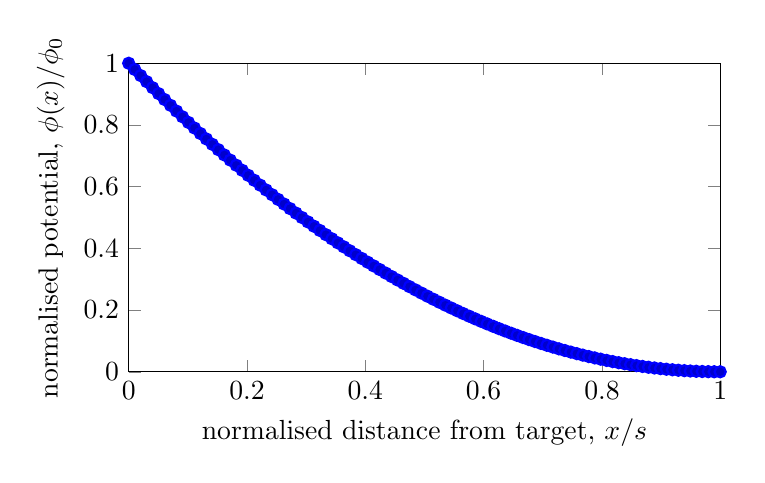
\begin{tikzpicture}
\begin{axis}[
 width=0.75\textwidth,
 height=5.5cm,
 xlabel={normalised distance from target, $x/s$},
 ylabel={normalised potential, $\phi(x)/\phi_{0}$},
 xmin=0, xmax=1, ymin=0, ymax=1,
 domain=0:1,
 samples=100,
 axis lines=box,
 every axis plot/.append style={thick, black},
]
\addplot {(1-x)^2};
\end{axis}
\end{tikzpicture}
\caption{Illustrative, purely analytic matrix-sheath potential profile $\phi(x)/\phi_{0} = (1-x/s)^{2}$, shown for orientation only; not fitted to, or derived from, any experimental data.}
\label{fig:sheath-profile}
\end{figure}

\section{Summary}

This chapter has specified a staged experimental programme for validating the ion energy flux framework developed earlier in this monograph. A dual-mode capacitive/inductive RF argon (with xenon and helium options) source provides an envelope spanning collisionless to weakly collisional sheath regimes. A four-port optical access geometry accommodates line-integrated interferometry, fibre-coupled OES, LIF, and incoherent Thomson scattering simultaneously, with provisions for stray-light rejection, window-fouling mitigation, and \'etendue-matched optics. The diagnostics are commissioned in a risk-ordered sequence -- OES and interferometry first, LIF second, Thomson scattering last -- so each more demanding technique is validated against an already-established baseline first. A factorial DOE matrix isolates the individual and joint effects of pressure, power, bias, and field on $\Gamma_{E}$, with built-in null tests, quasineutrality closure checks, and a mass-dependence falsifiability test from Equation~\eqref{ch20-eq:bohm}. A risk register maps every major failure mode onto an embedded mitigation, and feasibility rests not on the novelty of any single diagnostic but on precedent for each element of the chain, combined for the first time to close the measurement of $\Gamma_{E}$ across the plasma sheath.
